\documentclass[main.tex,fontsize=8pt,paper=a4,paper=portrait,DIV=calc,]{scrartcl}
% Document
\usepackage[T1]{fontenc}
\usepackage[dvipsnames]{xcolor}
\usepackage[nswissgerman,english]{babel}
\renewcommand{\familydefault}{\sfdefault}

% Format
\usepackage[top=5mm,bottom=1mm,left=5mm,right=5mm]{geometry}
%\setlength{\headheight}{\baselineskip}
%\setlength{\headsep}{0mm}

%\usepackage{scrlayer-scrpage}
%\clearpairofpagestyles
%\chead{{\bfseries\TITLE, \AUTHOR, \pagename~\thepage}}

%\addtokomafont{pagehead}{\upshape}

\usepackage{multicol}
\setlength{\columnsep}{2mm}
\setlength{\columnseprule}{0.1pt}

% Math
\usepackage{amsmath}
\usepackage{amssymb}
\usepackage{amsfonts}

% Code
\usepackage{fancyvrb, etoolbox, listings, xcolor}
%\usemintedstyle{bw}

%\newminted[shell]{bash}{
%fontsize=\footnotesize,
%fontfamily=tt,
%breaklines=true,
%frame=single,
%framerule=0.1pt,
%framesep=2mm,
%tabsize=2
%}
%\newminted{css}{
%breaklines=true,
%tabsize=4,
%autogobble=true,
%escapeinside=||,
%stripall=true,
%stripnl=true,
%}

    \definecolor{lightgray}{rgb}{0.95, 0.95, 0.95}
    \definecolor{darkgray}{rgb}{0.4, 0.4, 0.4}
    \definecolor{purple}{rgb}{0.65, 0.12, 0.82}
    \definecolor{ocherCode}{rgb}{1, 0.5, 0} % #FF7F00 -> rgb(239, 169, 0)
    \definecolor{blueCode}{rgb}{0, 0, 0.93} % #0000EE -> rgb(0, 0, 238)
    \definecolor{greenCode}{rgb}{0, 0.6, 0} % #009900 -> rgb(0, 153, 0)
    \definecolor{teal}{rgb}{0.0, 0.5, 0.5}

\lstdefinestyle{code}{
    identifierstyle=\color{black},
    keywordstyle=\color{blue}\bfseries\small,
    ndkeywordstyle=\color{greenCode}\bfseries\small,
    stringstyle=\color{ocherCode}\ttfamily\small,
    commentstyle=\color{teal}\ttfamily\textit\small,
    basicstyle=\ttfamily\small,
    breakatwhitespace=false,         
    breaklines=true,                 
    captionpos=b,                    
    keepspaces=true,                 
    showspaces=false,                
    showstringspaces=false,
    showtabs=false,                  
    tabsize=2,
    belowskip=-5pt
}



% Images
\usepackage{graphicx}
\newcommand{\pic}{\includegraphics[scale=0.3]}
\graphicspath{{Screenshots/}{../Screenshots}}
\makeatletter
\def\pictext#1#2{%
    \@ifnextchar[{%
    \pictext@iiiii{#1}{#2}%
    }{%
      \pictext@iiiii{#1}{#2}[0.5,0.4,0.3]% Default is 5
    }%
}
\def\pictext@iiiii#1#2[#3,#4,#5]{\begin{minipage}{#3\textwidth}\includegraphics[scale=#4]{#1}\end{minipage}\begin{minipage}{#5\textwidth}#2\end{minipage}}
\def\minipg#1#2{%
    \@ifnextchar[{%
    \minipg@iiii{#1}{#2}%
    }{%
      \minipg@iiii{#1}{#2}[0.3,0.6]% Default is 5
    }%
}
\def\minipg@iiii#1#2[#3,#4]{\vspace{0.8mm}\begin{minipage}{#3\textwidth}#1\end{minipage}\begin{minipage}{#4\textwidth}#2\end{minipage}{\vspace{0.8mm}}}
\makeatother

%\newenvironment{minty}[2]% environment name
%{% begin code
%  \begin{minipage}{#1}
%  \begin{minted}{#2}
%}%
%{% end code
%  \end{minted}
%  \end{minipage}
%  \end{minty}\ignorespacesafterend
%} 

% Smaller Lists
\usepackage{enumitem}
\setlist[itemize,enumerate]{leftmargin=3mm, labelindent=0mm, labelwidth=1mm, labelsep=1mm, nosep}
\setlist[description]{leftmargin=0mm, nosep}
\setlength{\parindent}{0cm}

% Smaller Titles
\usepackage[explicit]{titlesec}

%% Color Boxes
\newcommand{\sectioncolor}[1]{\colorbox{black!60}{\parbox{0.989\linewidth}{\color{white}#1}}}
\newcommand{\subsectioncolor}[1]{\colorbox{black!50}{\parbox{0.989\linewidth}{\color{white}#1}}}
\newcommand{\subsubsectioncolor}[1]{\colorbox{black!40}{\parbox{0.989\linewidth}{\color{white}#1}}}
\newcommand{\paragraphcolor}[1]{\colorbox{black!30}{\parbox{0.989\linewidth}{\color{white}#1}}}
\newcommand{\subparagraphcolor}[1]{\colorbox{black!20}{\parbox{0.989\linewidth}{\color{white}#1}}}

%% Title Format
\titleformat{\section}{\vspace{0.5mm}\bfseries}{}{0mm}{\sectioncolor{\thesection~#1}}[{\vspace{0.5mm}}]
\titleformat{\subsection}{\vspace{0.5mm}\bfseries}{}{0mm}{\subsectioncolor{\thesubsection~#1}}[{\vspace{0.5mm}}]
\titleformat{\subsubsection}{\vspace{0.5mm}\bfseries}{}{0mm}{\subsubsectioncolor{\thesubsubsection~#1}}[{\vspace{0.5mm}}]
\titleformat{\paragraph}{\vspace{0.5mm}\bfseries}{}{0mm}{\paragraphcolor{\theparagraph~#1}}[{\vspace{0.5mm}}]
\titleformat{\subparagraph}{\vspace{0.5mm}\bfseries}{}{0mm}{\subparagraphcolor{\thesubparagraph~#1}}[{\vspace{0.5mm}}]

%% Title Spacing
\titlespacing{\section}{0mm}{0mm}{0mm}
\titlespacing{\subsection}{0mm}{0mm}{0mm}
\titlespacing{\subsubsection}{0mm}{0mm}{0mm}
\titlespacing{\paragraph}{0mm}{0mm}{0mm}
\titlespacing{\subparagraph}{0mm}{0mm}{0mm}

%% format cells
\usepackage[document]{ragged2e}
\usepackage{array, makecell}
\renewcommand{\arraystretch}{2}
\newcommand{\mc}{\makecell[{{m{1\linewidth}}}]}



\begin{document}
\begin{table}[h!]
\section{Types of Projects}
\begin{tabular}{|m{0.205\linewidth}|m{0.75\linewidth}|}
\hline
\textbf{Serial Projects} & These projects are easy to manage, as they consist of existing products/workflows with a clear price and timeframe.\\
\hline
\textbf{Pioneer Projects} & These projects are hard to manage. They often include serious RND work and are often open-ended. Here a company needs to understand that the project may need more time/money than expected.\\
\end{tabular}
\subsection{Project Organization}
\begin{tabular}{|m{0.205\linewidth}|m{0.75\linewidth}|}
\hline
standard & In a standard organization the project manager is also the chief of said project. Members will be dedicated to this project.
The problem with this structure is the question of where do we get the people from? Internal departments often don't want to lose their workers and hiring external employees will also lead to problems.\\
\hline
Startup & The startup variant simply means creating a company just for this project. It solves the issues about employment, however this can only be done with projects that are big enough to justify a new company. \newline
There is also the problem of Department, you can't create a new company for a project that plays in the same space as your current other products.\\
\hline
\end{tabular}
\end{table}
\section{Project Management models}
\begin{table}[h!]
\begin{tabular}{|m{0,205\linewidth}|m{0.75\linewidth}|}
\hline
Agile vs Classic & 
Agile project management requires \textbf{a good team management}, however it provides a better change management, and it is the recommended structure for IT projects.\newline
Classic project management requires \textbf{a good Change management}, it handles teams easier, but changes are horrible for it, therefore it is not recommended for IT projects.\newline
Classic projects work with the \textbf{waterfall conecept}, this means that you can't go back when you have reached a milestone as \textbf{late changes would be too expensive}\newline
This is one of the main reasons as to why people prefer the agile concepts over the classic ones.\\
\hline
\end{tabular}
\subsection{Unified Process}
\begin{tabular}{|m{0.975\linewidth}|}
\hline
\minipg{
The Unified Process is an iterative development strategy that focuses agility over structure.\newline
It does this by first broadly defining the scope of the project and creating Domain Models that only feature the most important usecases.
These usecases will then be implemented, tested and given to people for feedback.\newline
Based on this feedback the phase 2 Domain Model will be created with new features that will be implemented.\newline We still focus only the most important ones.\newline
We do this until the project reaches a releasable state. \\}
{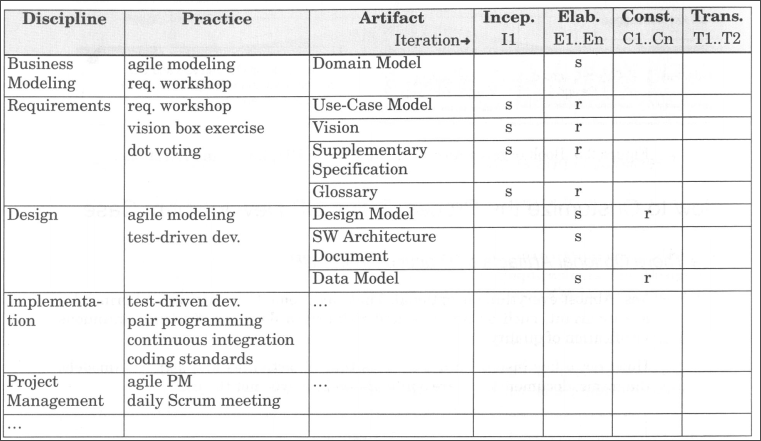
\includegraphics[scale=0.4]{2022-09-26-05_56_36.png}}[0.45,0.45]\\
\hline
\end{tabular}
\subsection{Phases of UP}
\begin{tabular}{|m{0,205\linewidth}|m{0.75\linewidth}|}
\hline
\textbf{\emph{Inception}} & Ceate a vision, scope, vague estimates and use cases.\\
\textbf{\emph{Elaboration}} & Create a refined vision, domain models, iterative implementation of core architecture, resolution of high risks, identification of most requirements and scope and more realistic estimates.\\
\textbf{\emph{Construction}} & Iterative implementation of remaining lower risk and easier elements, as well as preparation for deplyoment.\\
\textbf{\emph{Transition}} &beta tests and deplyoment \\
\hline
\end{tabular}
\subsection{CYNEFIN Framework}
\begin{tabular}{|m{0.2\linewidth}|m{0.755\linewidth}|}
\hline
\textbf{Complex} & 
\textcolor{red}{P-S-R}\newline
\textbf{Probe, Sense, Respond}\newline
\textcolor{green}{Emergent Practice}\\
\textbf{Complicated} & 
\textcolor{red}{S-A-R}\newline
\textbf{Sense, Analyze, Resond}\newline
\textcolor{green}{Good Practice}\\
\textbf{Chaotic} & 
\textcolor{red}{A-S-R}\newline
\textbf{Analyze, Sense, Respond}\newline
\textcolor{green}{Novel Practice}\\
\textbf{Simple} & 
\textcolor{red}{S-C-R}\newline
\textbf{Sense, Categorize, Respond}\newline
\textcolor{green}{Best Practice}\\
\hline
\end{tabular}
\subsection{HERMES Swiss trash}
\textbf{Handbuch der Elektronischen Rechenzentren des Bundes, eine Methode zur
Entwicklung von Systemen}
\begin{tabular}{|m{0.2\linewidth}|m{0.755\linewidth}|}
\hline
Category & HERMES is a classical project method, once again this shows why Switzerland just fucking sucks in terms of software engineering as they clearly focus on the wrong method.\newline
\minipg{
benefits:\newline
\begin{itemize}
\item high standardization
\item many tools in many languages
\item national certification
\item embedding of scrum
\item good for public institutions
\end{itemize}
}
{
negatives:\newline
\begin{itemize}
\item very constricted, not many freedoms
\item four phases, which are rather short
\item not relevant outside of switzerland, yay WHY EVEN PROPOSE THIS CRAP THEN?!
\item HERMES complicated projects...
\end{itemize}
}[0.25,0.5]\\
\hline
Phases & 
HERMES knows 4 phases:\newline
\begin{itemize}
  \item \textcolor{red}{Initialization} \textcolor{teal}{Goals, Requirements, Variants}
  \item \textcolor{red}{concepts} \textcolor{teal}{System requirements, Details, System architecture, prototypes}
  \item \textcolor{red}{Realization} \textcolor{teal}{Detailspecifications, system developed}
  \item \textcolor{red}{Introduction} \textcolor{teal}{system activated}
  \vspace{-3mm}
\end{itemize}\\
\hline
\end{tabular}
\end{table}
\begin{table}[h!]
\begin{tabular}{|m{0,205\linewidth}|m{0.75\linewidth}|}
\hline
SixSigma & 
\vspace{2mm}
\begin{itemize}
\item \textcolor{red}{\textbf{Define Measure Analyze Improve Control}}
\item \textcolor{orange}{Mathematical Model to measure and optimize processes}
\item \textcolor{orange}{independent of process or sector}
\item \textcolor{orange}{Shows how KPI is measured and how the process can be optimized by it}
\vspace{-3mm}
\end{itemize}\\
\hline
SixSigma Define &
\textcolor{red}{SIPOC -> Supplier - Input - Process - Output - Customer}\newline
\textcolor{orange}{SIPOC is the journey from the supplier to the customer, \newline
it defines what happens where in order to later on improve the workflow}\newline
\textcolor{red}{KOMY -> Key Output Measurement}\newline
\textcolor{orange}{KOMY is the formula that converts all input values to one output value.}\\
\hline
SixSigma Measure & 
\vspace{2mm}
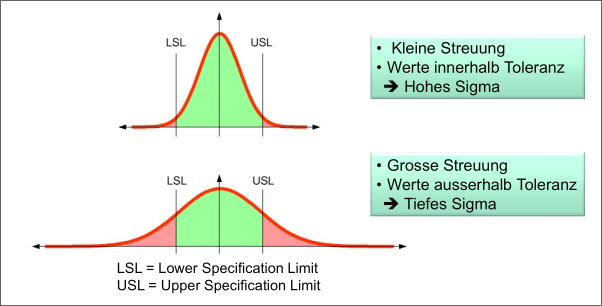
\includegraphics[scale=0.4]{2022-10-31-11_20_10.png}\\
\hline
SixSigma Improve & 
\textcolor{orange}{In order to improve you need 3 things:}\newline
\begin{itemize}
\item \textcolor{teal}{Knowledge and Skills}
\item \textcolor{teal}{Tools}
\item \textcolor{teal}{Mentality and Behavior}
\vspace{-3mm}
\end{itemize}\\
\hline
\end{tabular}
\section{Security Concept from CYSEC}
\begin{tabular}{|m{0.2\linewidth}|m{0.755\linewidth}|}
\hline
Confidentiality &
\textcolor{orange}{Information should only be available for users who need this information}\\
\hline
Integrity & 
\textcolor{orange}{Information is always \textbf{\textit{complete, trustworthy and secure}}}\\
\hline
Availability &
\textcolor{orange}{Systems are resilient against attacks and recover after error/crashes.}\\
\hline
Authenticity and Nonrepudation &
\textcolor{orange}{Every action can be traced back to the user who performed this action.}\\
\hline
\end{tabular}
\end{table}
\begin{table}[h!]
\begin{tabular}{|m{0,205\linewidth}|m{0.75\linewidth}|}
\hline

\hline
\end{tabular}
\end{table}
\end{document}

